\section{联合分布的分解}
\label{sec:cdis-joint}

上一节固定观测值，对条件分布积分。现在把观测值也放开，按观测的边缘分布再积分一次。概率表中，这相当于把条件分布的每一行乘回行的质量，恢复整张表；对列求和得到目标的边缘；逐个变量重复这一步，就能从头构造多个随机对象的联合规律。这一节依次落实这三件事，并说明每一步保留哪些条件变量。

\subsection{联合分布的恢复}
\label{sec:cdis-recovery}

引理~\ref{lem:cdis-regular-criterion}已经说明，矩形事件的联合概率可以由核与边缘恢复：
\[
 \mathbb{P}(X\in A,\ Y\in B)=\int_{B}K(y,A)\,P_Y(\mathrm{d}y).
\]
三角形模型中取$A=[\tfrac34,1]$、$B=[0,\tfrac12]$。对$y\leq\tfrac12$，$K(y,A)=\tfrac{1}{4(1-y)}$，乘以$f_Y(y)=2(1-y)$得到常数$\tfrac12$，所以
\[
 \mathbb{P}\bigl(X\geq\tfrac34,\ Y\leq\tfrac12\bigr)=\int_0^{1/2}\frac12\,\mathrm{d}y=\frac14 .
\]
直接计算，事件对应边长为$\tfrac14$与$\tfrac12$的矩形，它整个落在三角形内，面积$\tfrac18$乘以密度$2$也是$\tfrac14$，见图~\ref{fig:cdis-joint-recovery}。

\begin{BookInlineFigure}
  \centering
  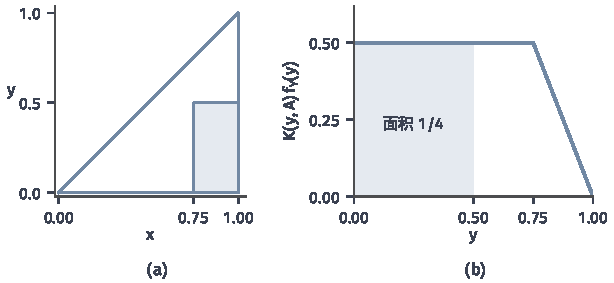
\includegraphics[width=104mm]{figures/07-probability/02-measure-theoretic-probability/matplotlib/cdis-joint-recovery/figure.pdf}
  \caption{由核与边缘恢复矩形事件的联合概率，三角形模型。(a)浅蓝矩形是事件$\{X\geq\tfrac34,\ Y\leq\tfrac12\}$，蓝线围成三角形。(b)蓝线是$y\mapsto K(y,A)f_Y(y)$，$A=[\tfrac34,1]$；它在$y\leq\tfrac34$时等于$\tfrac12$，此后等于$2(1-y)$。浅蓝区域是$[0,\tfrac12]$上的积分，面积为$\tfrac14$。}
  \label{fig:cdis-joint-recovery}
\end{BookInlineFigure}

矩形之外的事件，例如$\{X+Y\leq1\}$，以及一般的期望$\mathbb{E}[f(X,Y)]$，怎样由核与边缘算出？对乘积空间中的集合$E$，记它在$y$处的截面为$E^{y}=\{x:(x,y)\in E\}$。自然的猜测是先在每个$y$处按$K(y,\cdot)$量出截面，再按$Y$的分布累计。下面的定理说明这个猜测正确，并且由此定义的测度唯一。

\begin{theorem}[由核与边缘确定联合规律]
\label{thm:cdis-kernel-product}
设$\mu$是$\mathcal{Y}$上的概率测度，$K$是从$\mathcal{Y}$到$\mathcal{X}$的概率核。
\begin{enumerate}
 \item 对每个$E\in\mathcal{F}_{\mathcal{X}}\otimes\mathcal{F}_{\mathcal{Y}}$，$y\mapsto K(y,E^{y})$可测，并且
 \begin{equation}
  (\mu\otimes K)(E)=\int K(y,E^{y})\,\mu(\mathrm{d}y)
  \label{eq:cdis-kernel-product}
 \end{equation}
 是乘积空间上的概率测度。它是在每个可测矩形$A\times B$上取值$\int_{B}K(y,A)\,\mu(\mathrm{d}y)$的唯一概率测度。
 \item 对非负可测函数$f$，$y\mapsto\int f(x,y)\,K(y,\mathrm{d}x)$可测，并且
 \begin{equation}
  \int f\,\mathrm{d}(\mu\otimes K)=\int\!\!\int f(x,y)\,K(y,\mathrm{d}x)\,\mu(\mathrm{d}y).
  \label{eq:cdis-kernel-product-integral}
 \end{equation}
 若$f$关于$\mu\otimes K$可积，内层积分对$\mu$几乎每个$y$绝对收敛，式~\eqref{eq:cdis-kernel-product-integral}仍成立。
 \item 若$K$是给定$Y$时$X$的正则条件分布，则$P_Y\otimes K$就是$(X,Y)$的联合分布，从而对非负可测或使$f(X,Y)$可积的$f$，
 \begin{equation}
  \mathbb{E}[f(X,Y)]=\int\!\!\int f(x,y)\,K(y,\mathrm{d}x)\,P_Y(\mathrm{d}y).
  \label{eq:cdis-joint-recovery}
 \end{equation}
\end{enumerate}
\end{theorem}

\begin{proof}
第1条，先证可测性。令$\mathcal{D}$为使$y\mapsto K(y,E^{y})$可测的$E$的全体。对可测矩形，$(A\times B)^{y}$在$y\in B$时是$A$，否则是空集，所以$K(y,(A\times B)^{y})=K(y,A)\mathbf{1}_{B}(y)$可测，矩形属于$\mathcal{D}$。整个空间属于$\mathcal{D}$；补集的截面是截面的补集，$K(y,(E^{\mathrm{c}})^{y})=1-K(y,E^{y})$；两两不交的集合，截面也两两不交，$K(y,\cdot)$可数可加，所得的函数是可测函数之和。所以$\mathcal{D}$是$\lambda$系统。可测矩形对有限交封闭并生成乘积$\sigma$代数，由$\pi$--$\lambda$定理，$\mathcal{D}$包含全部可测集。

再证式~\eqref{eq:cdis-kernel-product}定义了概率测度。空集的截面都是空集，全空间的截面都是$\mathcal{X}$，所以测度分别为$0$和$1$。对两两不交的$E_n$，截面两两不交，
\[
 (\mu\otimes K)\Bigl(\bigcup_nE_n\Bigr)=\int\sum_{n}K(y,E_n^{y})\,\mu(\mathrm{d}y)=\sum_{n}(\mu\otimes K)(E_n),
\]
逐项积分的依据是单调收敛定理。取$E=A\times B$，式~\eqref{eq:cdis-kernel-product}给出$\int_{B}K(y,A)\,\mu(\mathrm{d}y)$。两个概率测度若在可测矩形上相同，由生成$\pi$系统上的唯一性，它们相同。

第2条，按积分的构造进行。$f=\mathbf{1}_{E}$时，内层积分是$K(y,E^{y})$，结论就是第1条。简单函数由线性得到。非负可测$f$取简单函数$f_n\uparrow f$：每个$y$处内层积分由单调收敛定理递增收敛，极限可测；外层再用一次单调收敛定理。$f$可积时，分别处理$f^{+}$与$f^{-}$；由非负情形，$\int\!\int\lvert f\rvert\,K(y,\mathrm{d}x)\,\mu(\mathrm{d}y)<\infty$，所以内层的$\int\lvert f(x,y)\rvert\,K(y,\mathrm{d}x)$只在$\mu$零测集上为无穷。

第3条，由引理~\ref{lem:cdis-regular-criterion}，$(X,Y)$的联合分布在每个可测矩形上的取值与$P_Y\otimes K$相同，由第1条的唯一性两者相同。式~\eqref{eq:cdis-joint-recovery}是第2条对联合分布的改写，其左边由分布的积分公式写成期望。
\end{proof}

定理与卷四的Tonelli、Fubini定理结构相同，可参考\BookChapterRef{chap:integration}{卷四第6章“积分”}。乘积测度是$K(y,\cdot)$不随$y$改变的特例：此时$\mu\otimes K$就是两个测度的乘积，$X$与$Y$独立。一般的核让截面的“量法”随$y$改变，这正是依赖关系的来源。

\paragraph{一个非矩形的例子}
用式~\eqref{eq:cdis-joint-recovery}计算三角形模型中的$\mathbb{E}[XY]$。内层对$x$积分时把$y$当作常数，由第~\ref{sec:cdis-integral-representation}小节，$\int x\,K(y,\mathrm{d}x)=(1+y)/2$，于是
\[
 \int x y\,K(y,\mathrm{d}x)=\frac{y(1+y)}{2}.
\]
再按$f_Y(y)=2(1-y)$积分，
\[
 \mathbb{E}[XY]=\int_0^1\frac{y(1+y)}{2}\cdot2(1-y)\,\mathrm{d}y=\int_0^1(y-y^{3})\,\mathrm{d}y=\frac14 .
\]
直接用联合密度计算，结果相同：
\[
 \int_0^1\int_0^{x}2xy\,\mathrm{d}y\,\mathrm{d}x=\int_0^1x^{3}\,\mathrm{d}x=\frac14 .
\]

\paragraph{给定观测时代入观测值}
定理~\ref{thm:cdis-kernel-product}还给出了一个常用的计算规则：求$f(X,Y)$给定$Y$的条件期望时，可以把$Y$的观测值代入，只对$X$按条件分布积分。设$\mathbb{E}\lvert f(X,Y)\rvert<\infty$，则
\begin{equation}
 \mathbb{E}[f(X,Y)\mid Y]=\int f(x,Y)\,K(Y,\mathrm{d}x)\quad\text{几乎必然}.
 \label{eq:cdis-substitution}
\end{equation}
右边由第2条是$Y$的可测函数。对$B\in\mathcal{F}_{\mathcal{Y}}$，把式~\eqref{eq:cdis-joint-recovery}用于$\mathbf{1}_{B}(y)f(x,y)$，得到右边在$\{Y\in B\}$上的积分等于$\mathbb{E}[\mathbf{1}_{\{Y\in B\}}f(X,Y)]$，这正是条件期望的积分刻画。例如$\mathbb{E}[XY\mid Y]=Y\,\mathbb{E}[X\mid Y]$，与提取已知量的规则一致。

\paragraph{不只是密度的乘法}
有联合密度时，式~\eqref{eq:cdis-joint-recovery}就是在$f_Y(y)>0$处把$f_{X,Y}$写成$f_Y(y)f_{X\mid Y}(x\mid y)$再作累次积分。定理本身不需要密度。图~\ref{fig:cdis-non-density}给出两个没有平面联合密度的例子。

\begin{BookInlineFigure}
  \centering
  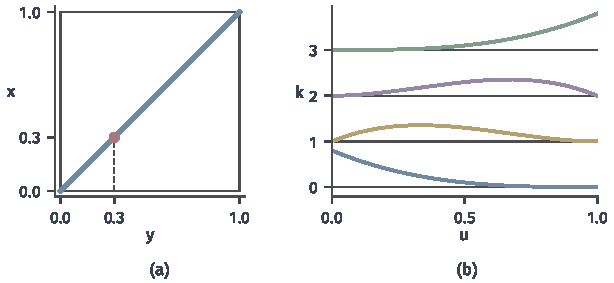
\includegraphics[width=104mm]{figures/07-probability/02-measure-theoretic-probability/matplotlib/cdis-non-density/figure.pdf}
  \caption{由核与边缘确定、但没有平面联合密度的联合规律。(a)$X=Y\sim\operatorname{Unif}(0,1)$：全部质量在蓝色对角线上，核$K(y,\cdot)=\delta_y$把$y=0.3$处的质量放在红点。(b)正面概率随机的硬币，$n=3$：$(U,N)$的质量分布在四条水平线$N=k$上，曲线是每条线上的密度$\binom{3}{k}u^{k}(1-u)^{3-k}$，$k=0,1,2,3$（蓝、黄、紫、绿）。}
  \label{fig:cdis-non-density}
\end{BookInlineFigure}

第一个例子是$X=Y\sim\operatorname{Unif}(0,1)$，核为$K(y,\cdot)=\delta_y$。由式~\eqref{eq:cdis-kernel-product}，$E^{y}$在$\delta_y$下的测度是$\mathbf{1}_{E}(y,y)$，所以
\[
 P_{(X,Y)}(E)=\int_0^1\mathbf{1}_{E}(y,y)\,\mathrm{d}y ,
\]
即质量沿对角线均匀分布。例如取$f(x,y)=(x-y)^{2}$，内层积分在每个$y$处都是$0$，所以$\mathbb{E}[(X-Y)^{2}]=0$。

第二个例子是硬币模型$(U,N)$，一个分量连续、一个分量离散。$N=k$的那条水平线上，质量关于$u$的密度是$\binom nk u^{k}(1-u)^{n-k}$；所有线上的密度对$u$积分再对$k$求和等于$1$。这两种联合规律都不是平面上的密度，却都由“边缘乘以核”唯一确定。

\subsection{全概率公式与混合分布}
\label{sec:cdis-mixture}

联合恢复公式中取$B=\mathcal{Y}$，即保留$X$的事件、对全部观测值积分，得到$X$的边缘分布：
\begin{equation}
 P_X(A)=\int K(y,A)\,P_Y(\mathrm{d}y),\qquad A\in\mathcal{F}_{\mathcal{X}} .
 \label{eq:cdis-total-probability}
\end{equation}
这是全概率公式的一般形式。第~\ref{chap:classical-probability}章的全概率公式把样本空间分成有限个正概率的组，再按组加权；这里的“组”是观测值$y$，可以有不可数多个，每组的概率可以为零，按$P_Y$加权的求和换成了积分。对函数，同样有$\mathbb{E}[g(X)]=\int(Kg)(y)\,P_Y(\mathrm{d}y)$，只要$g$非负或$g(X)$可积。

式~\eqref{eq:cdis-total-probability}也可以从另一个方向读：给定一族分布$\{K(y,\cdot)\}$和一个加权分布$\mu$，$\mu K$是一个新分布，称为这族分布按$\mu$的混合。$\mu$称为混合分布的权重，取值$y$称为混合变量。第~\ref{chap:random-vectors}章的房间温度模型就是两个分量的离散混合：$Y$表示房间状态，$\mu$给两种状态的概率$0.8$与$0.2$，$K$给出两个高斯分布，混合结果的密度是$0.8\,\phi(x-20)+0.2\,\phi(x-23)$。

\paragraph{连续混合：随机硬币的正面次数}
混合变量可以连续。硬币模型中，$U$的分布是$[0,1]$上的Lebesgue测度，代入式~\eqref{eq:cdis-total-probability}，
\[
 \mathbb{P}(N=k)=\int_0^1\binom nk u^{k}(1-u)^{n-k}\,\mathrm{d}u .
\]
由第~\ref{chap:common-distributions}章的Beta积分，对非负整数$a,b$，
\[
 \int_0^1u^{a}(1-u)^{b}\,\mathrm{d}u=\frac{a!\,b!}{(a+b+1)!},
\]
代入得到
\[
 \mathbb{P}(N=k)=\frac{n!}{k!\,(n-k)!}\cdot\frac{k!\,(n-k)!}{(n+1)!}=\frac{1}{n+1},\qquad k=0,1,\dots,n .
\]
正面次数在$\{0,1,\dots,n\}$上均匀分布。每个分量$\operatorname{Bin}(n,u)$都集中在$nu$附近，$u$均匀地扫过$[0,1]$，峰的位置也均匀地扫过$0$到$n$，叠加起来恰好铺平，见图~\ref{fig:cdis-mixtures}(a)。

\paragraph{连续混合：正态尺度混合}
第~\ref{chap:multivariate-distributions}章的多元t分布是另一个连续混合。那里$U\sim\chi^{2}_{\nu}$，给定$U=u$时$\bm{X}\sim\mathcal{N}\bigl(\bm{\mu},(\nu/u)\bm{\Sigma}\bigr)$，即核$K(u,\cdot)$是一族尺度不同的高斯分布。式~\eqref{eq:cdis-total-probability}给出
\[
 P_{\bm{X}}(S)=\int_0^{\infty}K(u,S)\,P_U(\mathrm{d}u),
\]
再对每个$K(u,\cdot)$的密度$g_u$用Tonelli定理交换积分，就得到那一章的混合密度：$\bm{X}$的密度是各分量密度$g_u(\bm{x})$按$P_U$的加权积分。这里的推导不需要$U$有密度：把尺度的分布换成任何$(0,\infty)$上的分布，例如只取两个值，混合仍有密度，只要每个分量有密度且$u\mapsto g_u(\bm{x})$可测。

\begin{BookInlineFigure}
  \centering
  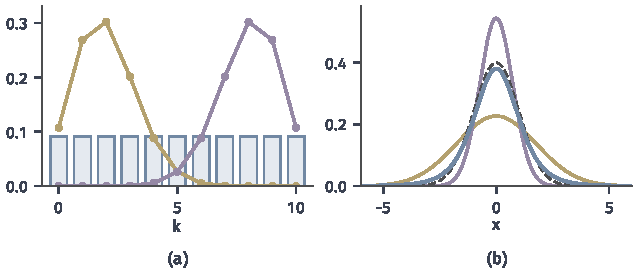
\includegraphics[width=108mm]{figures/07-probability/02-measure-theoretic-probability/matplotlib/cdis-mixtures/figure.pdf}
  \caption{两个连续混合。(a)$n=10$时的两个分量$\operatorname{Bin}(10,u)$，$u=0.2$（黄）与$u=0.8$（紫），以及对$u\in[0,1]$均匀混合后的分布，各点概率都是$1/11$（浅蓝柱）。(b)一元t分布作为正态尺度混合，$\nu=5$：黄、紫线是$U$取$\chi^{2}_{5}$的$10\%$与$90\%$分位数时的分量$\mathcal{N}(0,5/u)$，蓝线是混合得到的t密度，灰色虚线是$\mathcal{N}(0,1)$。}
  \label{fig:cdis-mixtures}
\end{BookInlineFigure}

图~\ref{fig:cdis-mixtures}(b)中，$u$较小的分量又宽又矮，$u$较大的分量窄而高；混合后的t密度中心比标准高斯略低，尾部明显更厚，厚尾来自那些尺度很大的分量。混合分布的矩也按条件矩加权：均值是条件均值的平均，方差由全方差公式分成组内与组间两部分，第~\ref{sec:cdis-conditional-moments}小节的硬币例子就是一次具体的计算。

\subsection{链式分解}
\label{sec:cdis-chain}

两个随机对象的联合规律可以分成“先$Y$、再给定$Y$的$X$”两步。有$n$个随机对象$X_1,\dots,X_n$时，可以依次进行：先定$X_1$，再给定$X_1$定$X_2$，再给定$(X_1,X_2)$定$X_3$，如此下去。每一步需要一个正则条件分布，它的存在由定理~\ref{thm:cdis-existence}保证，这里要求每个$X_k$取值于标准Borel空间$\mathcal{X}_k$。

记$\bm{x}_{1:k}=(x_1,\dots,x_k)$，$X_{1:k}=(X_1,\dots,X_k)$。下面的定理用到一个事实：标准Borel空间的有限乘积仍是标准Borel空间，这是第~\ref{sec:cdis-existence-conditions}小节所述可数乘积结论的特例。

\begin{theorem}[链式分解]
\label{thm:cdis-chain}
设$X_1,\dots,X_n$分别取值于标准Borel空间$\mathcal{X}_1,\dots,\mathcal{X}_n$。则存在概率核$K_k$（$k=2,\dots,n$），$K_k$从$\mathcal{X}_1\times\cdots\times\mathcal{X}_{k-1}$到$\mathcal{X}_k$，是给定$X_{1:k-1}$时$X_k$的正则条件分布；并且对非负可测函数$f$，
\begin{equation}
 \mathbb{E}[f(X_{1:n})]=\int P_{X_1}(\mathrm{d}x_1)\int K_2(x_1,\mathrm{d}x_2)\cdots\int K_n(\bm{x}_{1:n-1},\mathrm{d}x_n)\,f(\bm{x}_{1:n}).
 \label{eq:cdis-chain}
\end{equation}
反过来，任给$\mathcal{X}_1$上的概率测度$P_1$和这样的一列概率核$K_2,\dots,K_n$，式~\eqref{eq:cdis-chain}的右边（取$f$为指示函数）定义了乘积空间上唯一的概率测度；在这个测度下，坐标$X_1$的分布是$P_1$，$K_k$是给定$X_{1:k-1}$时$X_k$的正则条件分布。
\end{theorem}

\begin{proof}
对$n$归纳。$n=1$时式~\eqref{eq:cdis-chain}是分布的积分公式。设结论对$n-1$成立。$X_{1:n-1}$取值于标准Borel空间$\mathcal{X}_1\times\cdots\times\mathcal{X}_{n-1}$，由定理~\ref{thm:cdis-existence}，给定$X_{1:n-1}$时$X_n$的正则条件分布$K_n$存在。由定理~\ref{thm:cdis-kernel-product}第3条，取$Y=X_{1:n-1}$、$X=X_n$，
\[
 \mathbb{E}[f(X_{1:n})]=\int\Bigl(\int f(\bm{x}_{1:n-1},x_n)\,K_n(\bm{x}_{1:n-1},\mathrm{d}x_n)\Bigr)P_{X_{1:n-1}}(\mathrm{d}\bm{x}_{1:n-1}).
\]
括号内是$\bm{x}_{1:n-1}$的非负可测函数，对它用归纳假设展开外层积分，就得到式~\eqref{eq:cdis-chain}。

反方向同样归纳：由$P_1$与$K_2$，定理~\ref{thm:cdis-kernel-product}第1条给出$\mathcal{X}_1\times\mathcal{X}_2$上唯一的测度$\mu_2=P_1\otimes K_2$；再由$\mu_2$与$K_3$得到$\mu_3=\mu_2\otimes K_3$，依此类推。每一步的唯一性来自第1条。在$\mu_k$下，由第1条中的矩形公式与引理~\ref{lem:cdis-regular-criterion}，$K_k$是给定前$k-1$个坐标时第$k$个坐标的正则条件分布；后面各步只在前$k$个坐标之外添加新坐标，不改变前$k$个坐标的联合分布。
\end{proof}

正向的结论说，任何有限个标准Borel随机对象的联合规律都能逐次分解；反向的结论说，可以用起始分布和一列核逐步构造联合规律：先按$P_1$抽$x_1$，再按$K_2(x_1,\cdot)$抽$x_2$，再按$K_3(x_1,x_2,\cdot)$抽$x_3$。每一步的核都可以依赖已经得到的\emph{全部}取值。按这种方式实际产生样本的方法在第~\ref{chap:sample-generation}章研究。有联合密度时，式~\eqref{eq:cdis-chain}就是密度的连乘分解
\[
 f(\bm{x}_{1:n})=f_{X_1}(x_1)\,f_{X_2\mid X_1}(x_2\mid x_1)\cdots f_{X_n\mid X_{1:n-1}}(x_n\mid\bm{x}_{1:n-1}),
\]
在各边缘密度为正的范围内成立。

\paragraph{随机硬币的逐次抛掷}
回到正面概率为$U\sim\operatorname{Unif}(0,1)$的硬币，记第$k$次的结果为$X_k\in\{0,1\}$，$1$表示正面，给定$U=u$时各次独立且$\mathbb{P}(X_k=1\mid U=u)=u$。前$m$次中正面有$s$次的某个具体结果序列，概率是
\[
 \mathbb{P}(X_{1:m}=\bm{x}_{1:m})=\int_0^1u^{s}(1-u)^{m-s}\,\mathrm{d}u=\frac{s!\,(m-s)!}{(m+1)!}.
\]
它只依赖正面次数$s$，与正反面出现的次序无关。

给定前$k-1$次的结果，其中正面$s$次，第$k$次为正面的条件概率是两个这样的概率之比，取$m=k-1$：
\begin{equation}
 \mathbb{P}(X_k=1\mid X_{1:k-1}=\bm{x}_{1:k-1})=\frac{(s+1)!\,(k-1-s)!/(k+1)!}{s!\,(k-1-s)!/k!}=\frac{s+1}{k+1}.
 \label{eq:cdis-succession}
\end{equation}
这称为\term{Laplace继承法则}（Laplace's rule of succession）。先看到的正面越多，下一次越可能是正面：抛掷结果在不断透露$U$的信息。由于每个$\bm{x}_{1:k-1}$的概率为正，这里的核由初等条件概率唯一确定。

用链式分解计算$\mathbb{P}(X_1=1,X_2=1,X_3=0)$。三个因子依次由式~\eqref{eq:cdis-succession}取$k=1,2,3$得到：
\[
 \begin{gathered}
 \mathbb{P}(X_1=1)=\frac12,\qquad \mathbb{P}(X_2=1\mid X_1=1)=\frac23,\\
 \mathbb{P}(X_3=0\mid X_1=1,X_2=1)=1-\frac34=\frac14 .
 \end{gathered}
\]
相乘得到$\tfrac1{12}$，与直接积分的结果相同：
\[
 \int_0^1u^{2}(1-u)\,\mathrm{d}u=\frac13-\frac14=\frac1{12}.
\]
图~\ref{fig:cdis-succession-tree}画出全部八条路径。

\begin{BookInlineFigure}
  \centering
  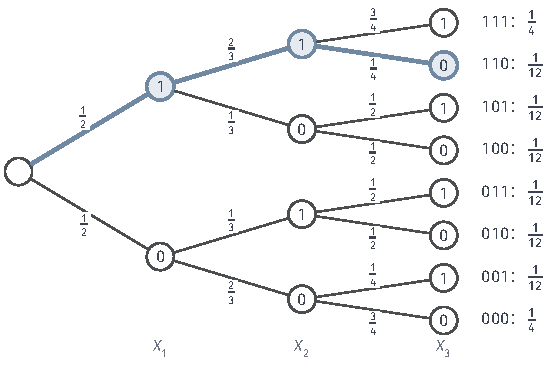
\includegraphics[width=94mm]{figures/07-probability/02-measure-theoretic-probability/tikz/cdis-succession-tree/figure.pdf}
  \caption{随机硬币前三次抛掷的链式分解。每条边上是由Laplace继承法则得到的条件概率，右侧是八个结果序列的概率；蓝色路径是$(1,1,0)$，概率为$\tfrac12\cdot\tfrac23\cdot\tfrac14=\tfrac1{12}$。}
  \label{fig:cdis-succession-tree}
\end{BookInlineFigure}

\paragraph{省去条件变量的后果}
式~\eqref{eq:cdis-chain}中每个核都给定了此前的全部变量。若为了简便，第三步只用$X_2$而忽略$X_1$，计算会出错。三次抛掷的联合规律在交换次序后不变，所以$(X_2,X_3)$与$(X_1,X_2)$同分布，
\[
 \mathbb{P}(X_3=0\mid X_2=1)=\mathbb{P}(X_2=0\mid X_1=1)=\frac13 ,
\]
于是“省略版”给出
\[
 \frac12\cdot\frac23\cdot\frac13=\frac19\neq\frac1{12}.
\]
差别的来源是：$X_1=1$与$X_2=1$合起来比单独的$X_2=1$透露了更多关于$U$的信息，使下一次出现反面的可能更小。图~\ref{fig:cdis-chain-omit}比较了八个序列在两种算法下的概率。省略版仍然给出一个总和为$1$的分布，所以无法从归一性看出错误。

\begin{BookInlineFigure}
  \centering
  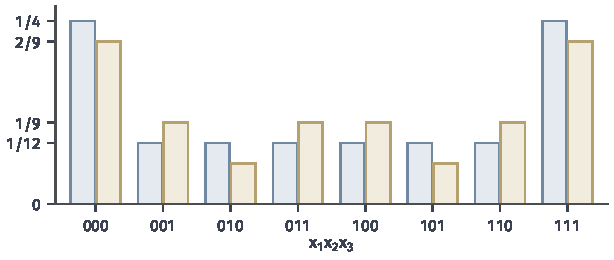
\includegraphics[width=104mm]{figures/07-probability/02-measure-theoretic-probability/matplotlib/cdis-chain-omit/figure.pdf}
  \caption{随机硬币三次抛掷的八个结果序列。蓝柱是由完整链式分解得到的真实概率，黄柱是第三步只给定$X_2$时的“省略版”概率；两组各自的和都是$1$，但在每个序列上都不相同。}
  \label{fig:cdis-chain-omit}
\end{BookInlineFigure}

一般地，把$K_k(\bm{x}_{1:k-1},\cdot)$换成只依赖其中一部分变量的核，是一个需要证明的断言：给定那部分变量以后，被省去的变量对$X_k$不再提供信息。这正是下一节的条件独立。
